\documentclass{article}
\usepackage[utf8]{inputenc}
\usepackage{graphicx}
\begin{document}
\title{Capita selecta III: Protexted-Module Architectures} 
\author{André Jacobs\\ r0370664}
\date{}
\maketitle
\section{Implementing a vault}

\subsection{Give three example use cases where SGX enclaves can provide a significant
security advantage}

\begin{itemize}
  \item Cryptograhic keys: cryptographic keys are essential when trying to
    encrypt data securely. Key management is an important and sometimes
    difficult aspect of keeping data secure. In general it is prefered to store
    cryptographic keys in hardware, and not in software. At the moment this
    requires special hardware that has been initialized during production. Protected software
    modules would allow to store any cryptographic key in hardware.
  \item DRM (digital rights management): companies that do not want their
    software products to be spread or reverse engineerd can use an enclave to
    protect and execute the most important parts of their code. 
  \item Extensible networked systems: nowadays computing devices are everywhere
    and often they are connected through several networks and support
    extensibility by third parties. In order to provide security for these
    devices and between the several software extensions, intel sgx enclaves can
    be used to prvent interference between code. One of the main advantages is
    that developers have to trust less of the software stack as they can rely on
    hardware protection.
\end{itemize}

\subsection{How is this enclave bootstrapped?  Where does the secret initially come
from?  How can the secret be provided securely to the enclave?}
First the OS requests for space in memory and loads Enclave code. Next the memoryspace for the protected code is marked as protected
and access control is enabled for that addressrange. Lastly the internal
datastructures of the Enclave are initialized. 

The secret in the vault is initially provided by public data (hardcoded in the
sourcode). This is actually
not very secure and only usable when secure execution is wanted, and not
secrecy.

A more secure way would be to use a cryptographically encrypted and signed file
which contains the secret. The key that is used to encrypt and sign the vault
should be the key from the key deriviation functionality, which is based on
Enclave properties. This way different instances of the same Enclave can access
the secret.
To initialize the secret file, the bootstrap process should create this file as soon
as possible and it's secret data should be provided directly by hardware,
copying from protected memory so it can only be accessed at boot time.


\subsection{It is obvious why an attacker should not be able to directly access the
stored secret, but why do we need to define what the entry points are?
What could go wrong?}
The intel sgx hardware makes it possible to protect a certain part of the
memory. Once inside the enclave it is possible to exectute all code in that
memory range. There must be a secure way to access this trusted code. The
trusted code requires input to interact with the secret. The hardware cannot
magically protect against every kind of attack, it only isolates code. Thus it's
the programmers responsibity to validate the user input. Without well defined
entrypoints, programmers cannot do proper validation checks.

\subsection{When the enclave is created, what prevents an attacker from adding a new
entry point that returns the secret
without
requiring the correct password.
How can such situations be detected?}

Intel sgx contain a key deriviation mechanism to prevent this from happening.
This key is derived from properties of the module, including it's measurements.
This means that only identical modules can generate the same key. If an attacker
were to modify the enclave before the enclave was created, then the
cryptographic key would not match anymore.

\section{Badly written EDL-files}
\subsection{After a user/attacker provides 3 incorrect passwords, she should be locked
  out indefinitely.  Is this implemented correctly in the pseudocode or your
implementation?  What can go wrong?  How did you fix the vulnerability?}

No, the hacker can still attempt to provide a password, and lower the
\texttt{numer\_of\_tries\_left} counter. This will result in an integer
overflow. While officially this is defined as undefined behaviour, on many
modern machine's using 2-complement representation this can result in a wrap
around, making the variable positive again. If that's not the case, it can simply
crash the program. This is also not wanted behaviour. Especially if state
continuity is not guarantueed.

This vulnerability can be solved by moving the decrement operation to the else
branch of the check. Or by returning immediately when the counter is 0.

\subsection{How did you trick the enclave into providing you with the secret, even
  though you didn’t know the correct password?   Draw an image of the
  memory layout and describe what happened.  In case you didn’t manage
to extract the secret, explain what you tried to do.}

The \texttt{get\_correct\_password\_address} returns a pointer to an address in
the isolated memory space. It is not possible to read these addresses
in the untrusted part of the code. Providing this pointer to an entrypoint is
still possible. It would be up to the programmer to check this input. 

When providing the pointer to the password's address as the \texttt{output}
parameter, it will be overridden as the empty string when a wrong password is
provided. Hence later we can try to access the secret with an empty password.

  \begin{figure}
    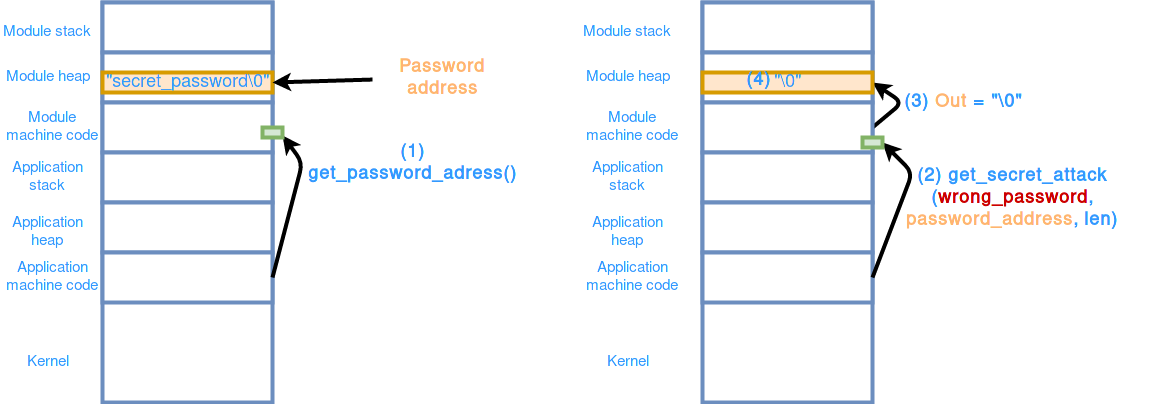
\includegraphics[width=0.99\textwidth]{./sgx.png}
  \end{figure}

\subsection{The newly added
  get
  secret
  attack
  entry point casts an
  uint64\_t
  to
  a
  char *
  .  Why is this necessary.  Does your attack still work when you
  use a
  char *
  .  Why not?  }

  This is necessary because when using the \texttt{[in, string]}-check in the
  \texttt{edl-file}, the edgr8r tool writes a check on
  pointers to a string (method \texttt{CHECK\_REF\_POINTER} checks
    \texttt{sgx\_is\_outside\_enclave}). It checks if the pointer does not point to protected
  memory. Changing the parameter to an int, removes the possibilty to perform
  this check. That is why it is not
  possible to simply provide the address as a \texttt{char*} as the provided
  password, since we would always need it to me a string (\texttt{char*}) to do
  a string comparison.

\subsection{Propose how to make the enclave keep its state over reboots.  What are
the security challenges?}

In order to keep state continuity, the Enclave should store it's
state on disk. It can do this safely by using the earlier discussed derived key.
In addition it requires the use of two principles: (1) Storing state+input before it
is processed and (2) any non-determinism should be treated as input and trigger
a storing of state.


\end{document}
